%%%%%%%%%%%%%%%%%%%%%%%%%%%%%%%%%%%%%%%%%%%%%%%%%%%%%%%%%%%%%%%%%%%%%%%%
%                                                                      %
%     File: Thesis_Appendix_A.tex                                      %
%     Tex Master: Thesis.tex                                           %
%                                                                      %
%     Author: Andre C. Marta                                           %
%     Last modified :  2 Jul 2015                                      %
%                                                                      %
%%%%%%%%%%%%%%%%%%%%%%%%%%%%%%%%%%%%%%%%%%%%%%%%%%%%%%%%%%%%%%%%%%%%%%%%

\chapter{Softdrop mass}
\label{chapter:SDmass}

Ii is noticeable in the softdrop mass spectrum of both Higgs candidates (for signal and backgrounds) the existence an atypical peak close to zero. In this section we explain the origin of this feature.

We believe that the peak close to zero corresponds to Higgs candidates ($R=0.8$ jets) that do not contain both b quarks from the Higgs decay. The plot that supports this conclusion is shown in figure \ref{fig:SDmass_peak}. It shows the correlation between the maximum $\Delta R$ between the Higgs candidate jet axis and one of the b quarks (y axis) and the jet's mass (x axis). The horizontal line corresponds to $\Delta R=0.8$. For small masses ($<80$ GeV) the maximum $\Delta R$ is usually larger than $0.8$ which means that at least one of the b quarks is not contained in the jet's cone. When applying the soft drop procedure to these jets, soft radiation is removed and we are left with a single b quark. The mass of b quarks is $\sim5$ GeV and therefore we get a peak at this mass.

In practice, this does not affect our analysis because we place a mass window cut around the Higgs boson mass and therefore the low mass peak is removed. Nonetheless, the study presented here is extremely important because it helps rule out possible malfunctions of the soft drop algorithm and gives us confidence that we understand exactly what is happening. 

\begin{figure}
	\centering
	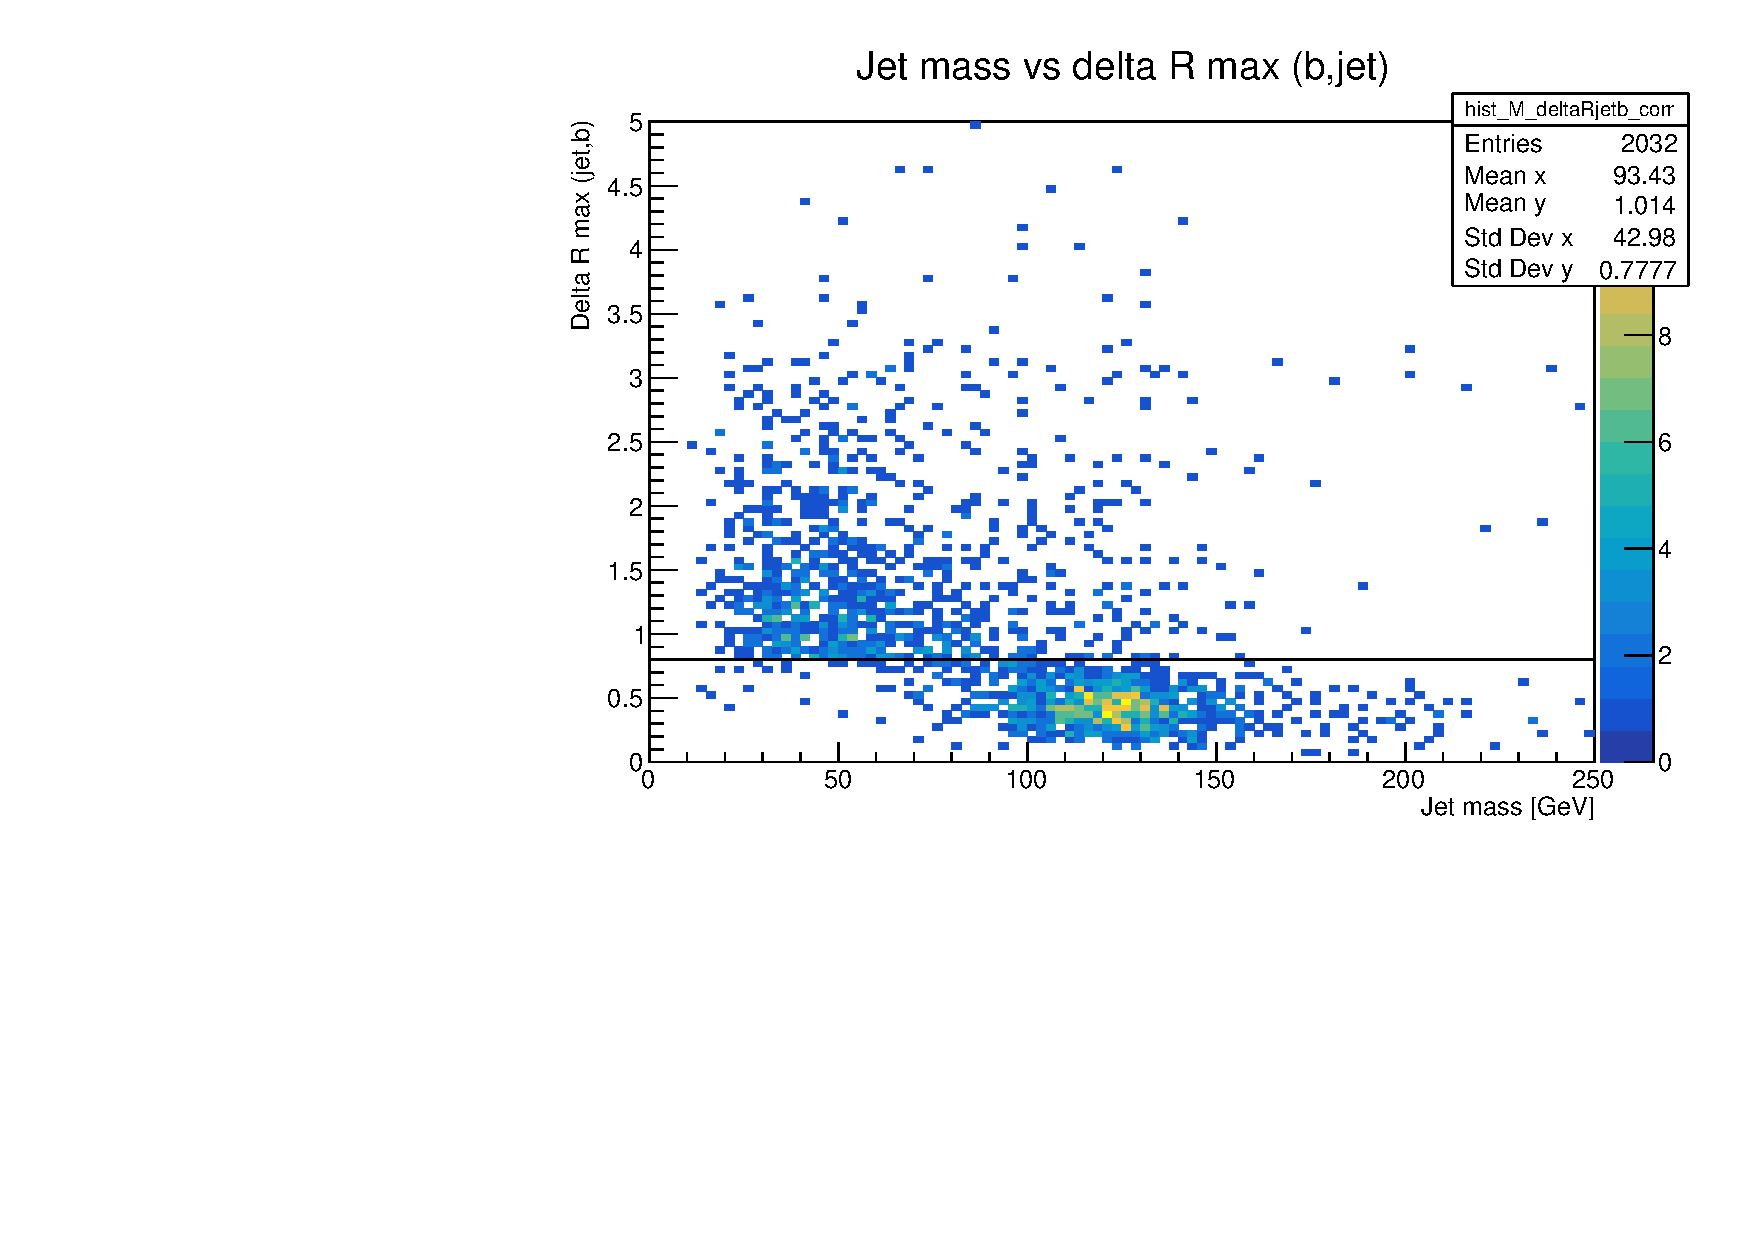
\includegraphics[width=0.5\textwidth]{./Figures/hist_M_deltaRmax_jetb_corr.pdf}
	\caption{Correlation between the maximum $\Delta R$ between the Higgs candidate jet and one of the b quarks (y axis) and the jet's mass (x axis). The horizontal line corresponds to $\Delta R=0.8$.}
	\label{fig:SDmass_peak}
\end{figure}
